\documentclass[border=2mm]{standalone}
\usepackage{tikz}
\usepackage{graphicx}

% Define common parameters
\newcommand{\imgwidth}{2cm}
\newcommand{\imgheight}{2cm}

% Define styles
\tikzset{
ssvep label/.style={above},
ssvep arrow/.style={ultra thick, ->},
image node/.style={above, midway, inner sep=0},
}

\begin{document}
\begin{tikzpicture}[xscale=2, yscale=1.5]
        
    % draw vertical ticks and labels
    \foreach \x/\label in {0/0,3/3,6/6,9/9, 12/12} {
    \draw (\x,0.2) -- (\x,-0.2);
    \node[below] at (\x,-0.2) {\label};
    }
    
    \fill[black!10] (3,0) rectangle (9,6);
    \fill[black!25] (3,4) rectangle (9,6);
    \fill[black!10] (12,0) rectangle (13,6);
    \fill[black!25] (12,2) rectangle (13,4);
    
    
    \draw[color=white, ultra thick]
    (0,0) -- (3,0) node[above,midway] { 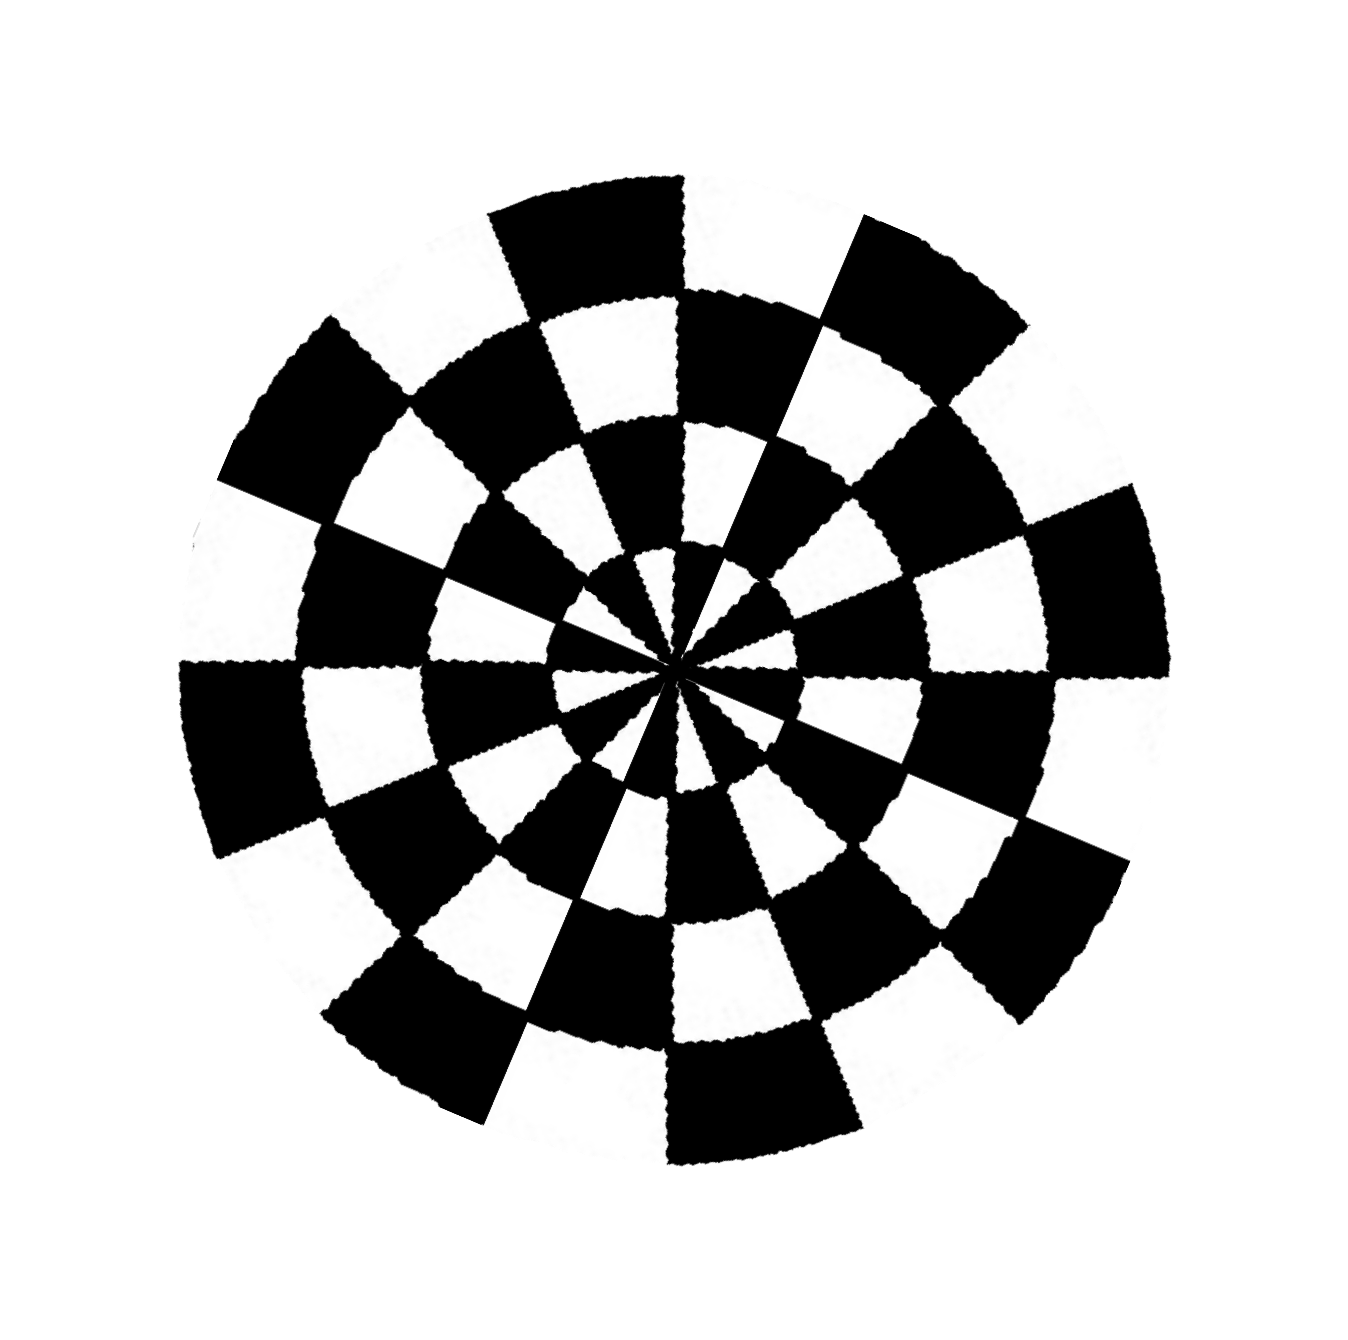
\includegraphics[width=2cm,height=2cm]{experiments/pattern.png}}
    (3,0) -- (6,0) node[above,midway] {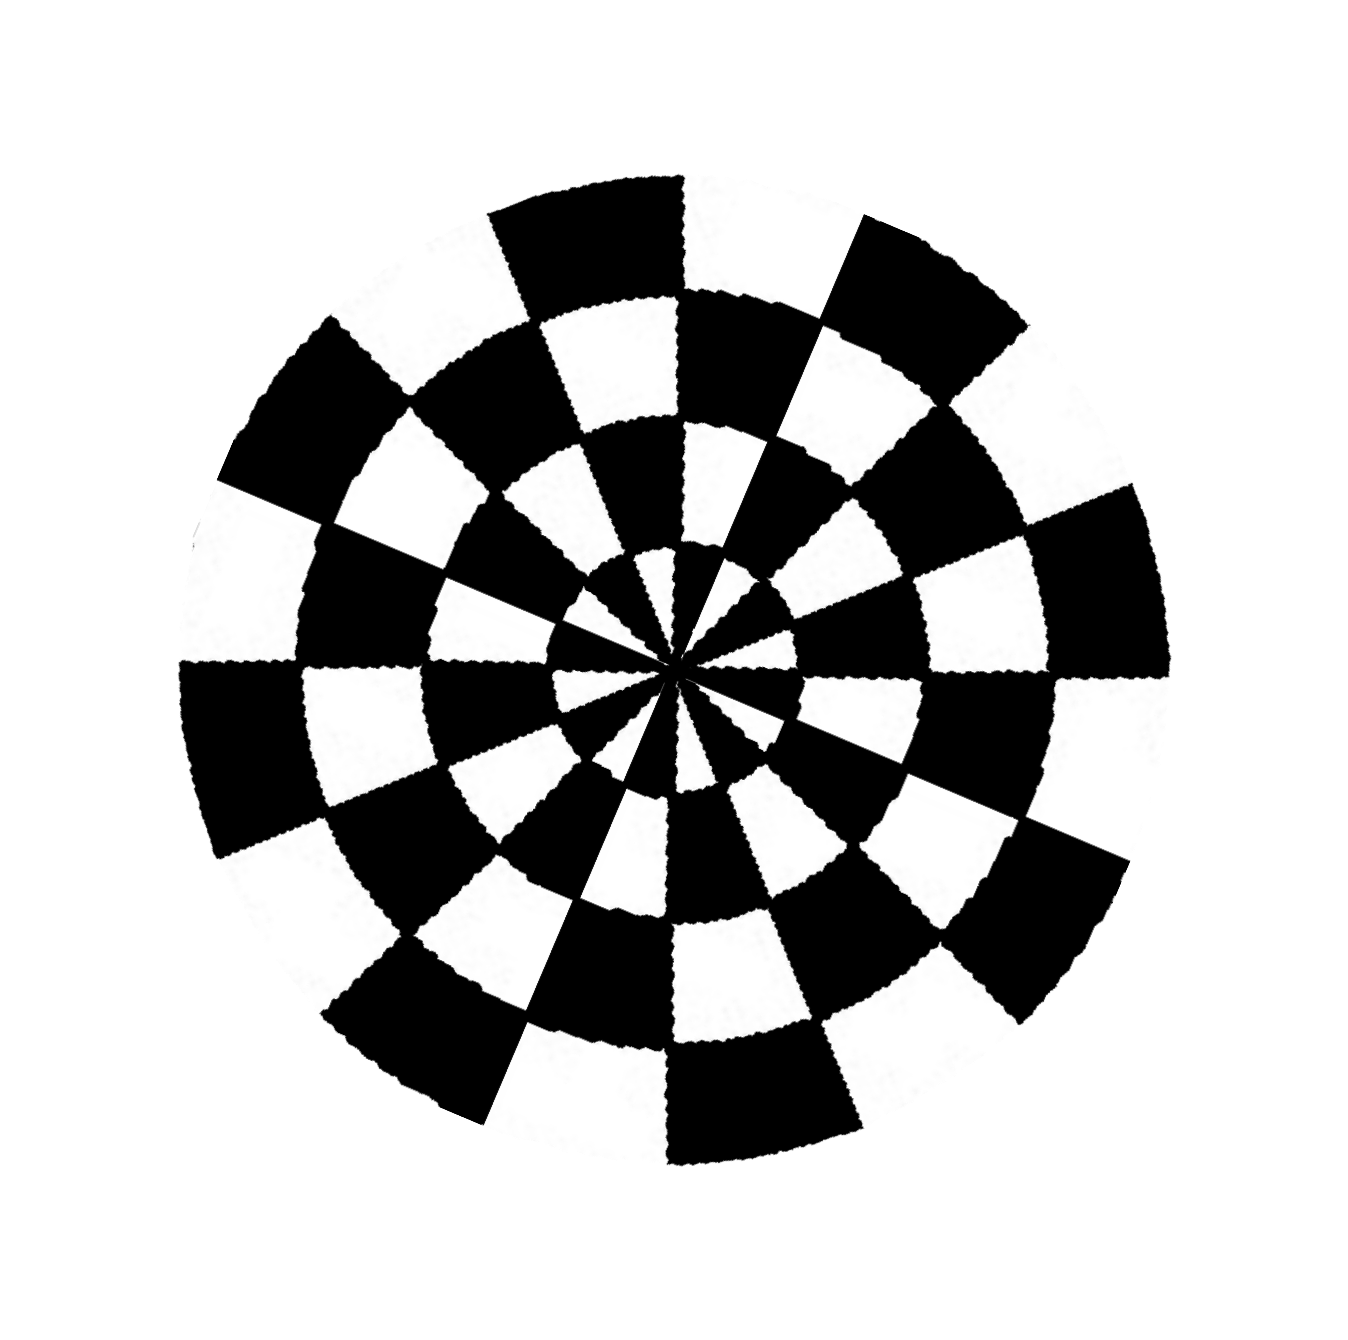
\includegraphics[width=2cm,height=2cm]{experiments/pattern.png}} 
    (6,0) -- (9,0) node[above, midway] {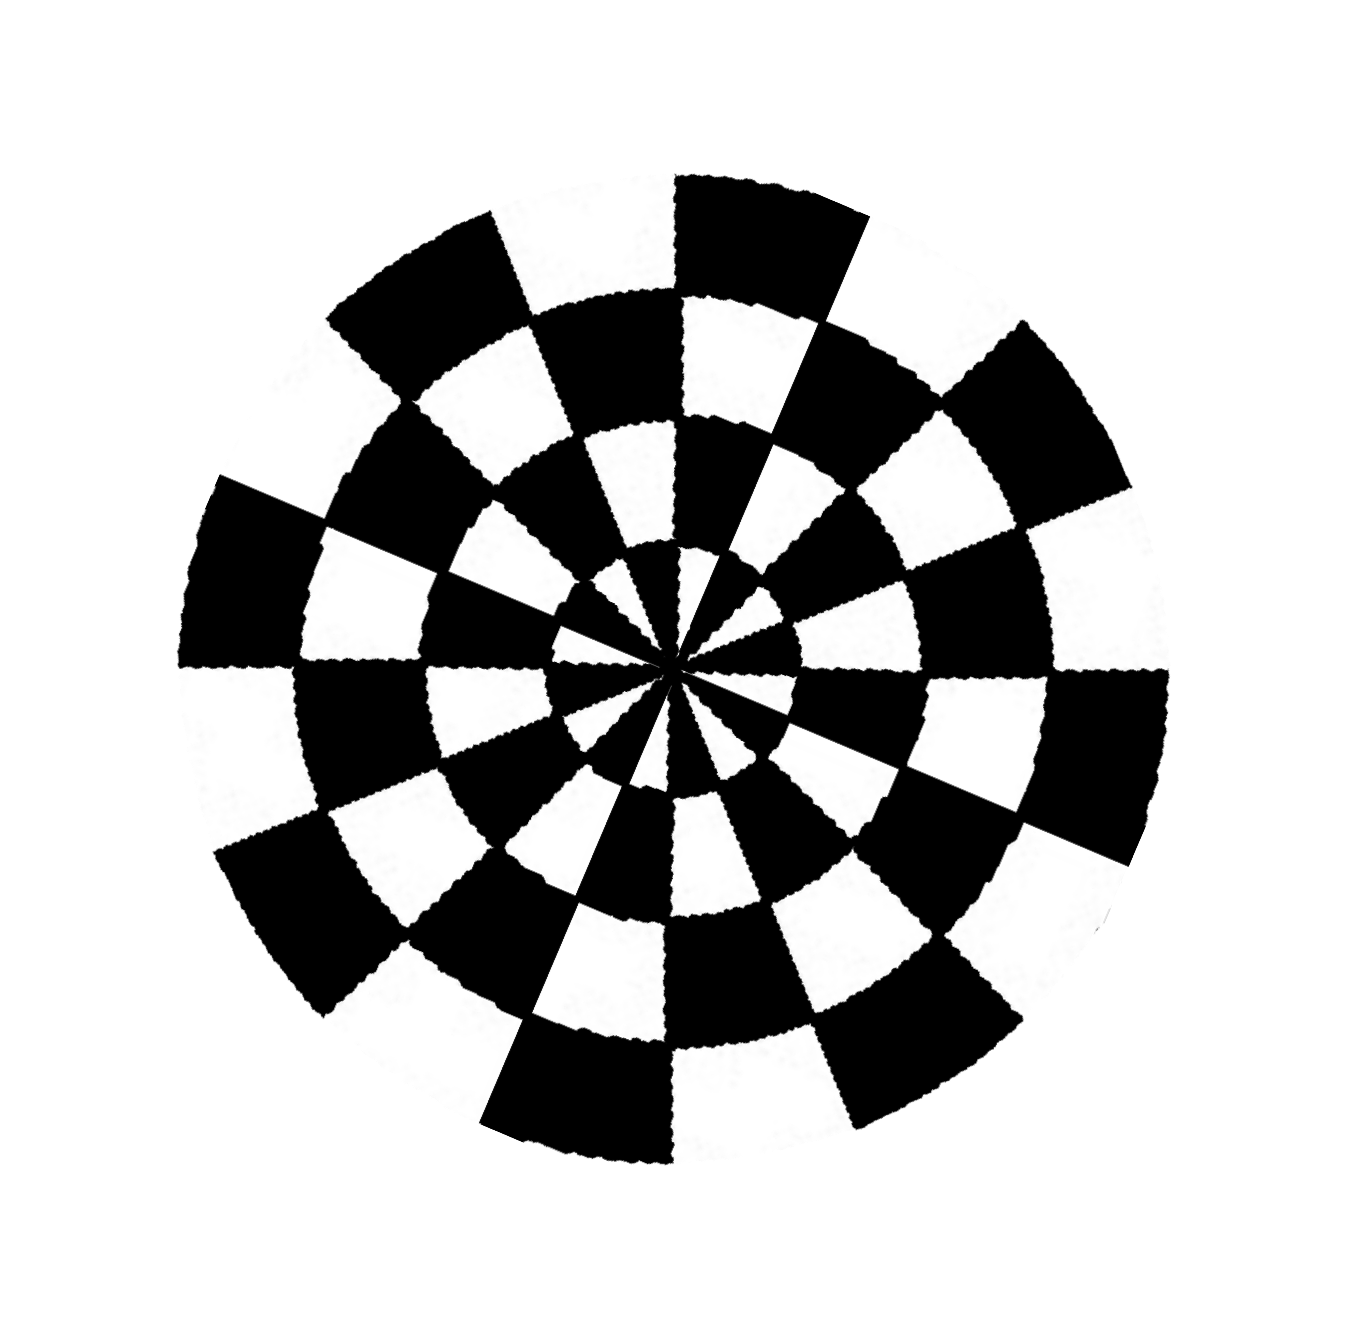
\includegraphics[width=2cm,height=2cm]{experiments/pattern_f.png}}
    (9,0) -- (12,0) node[above, midway] {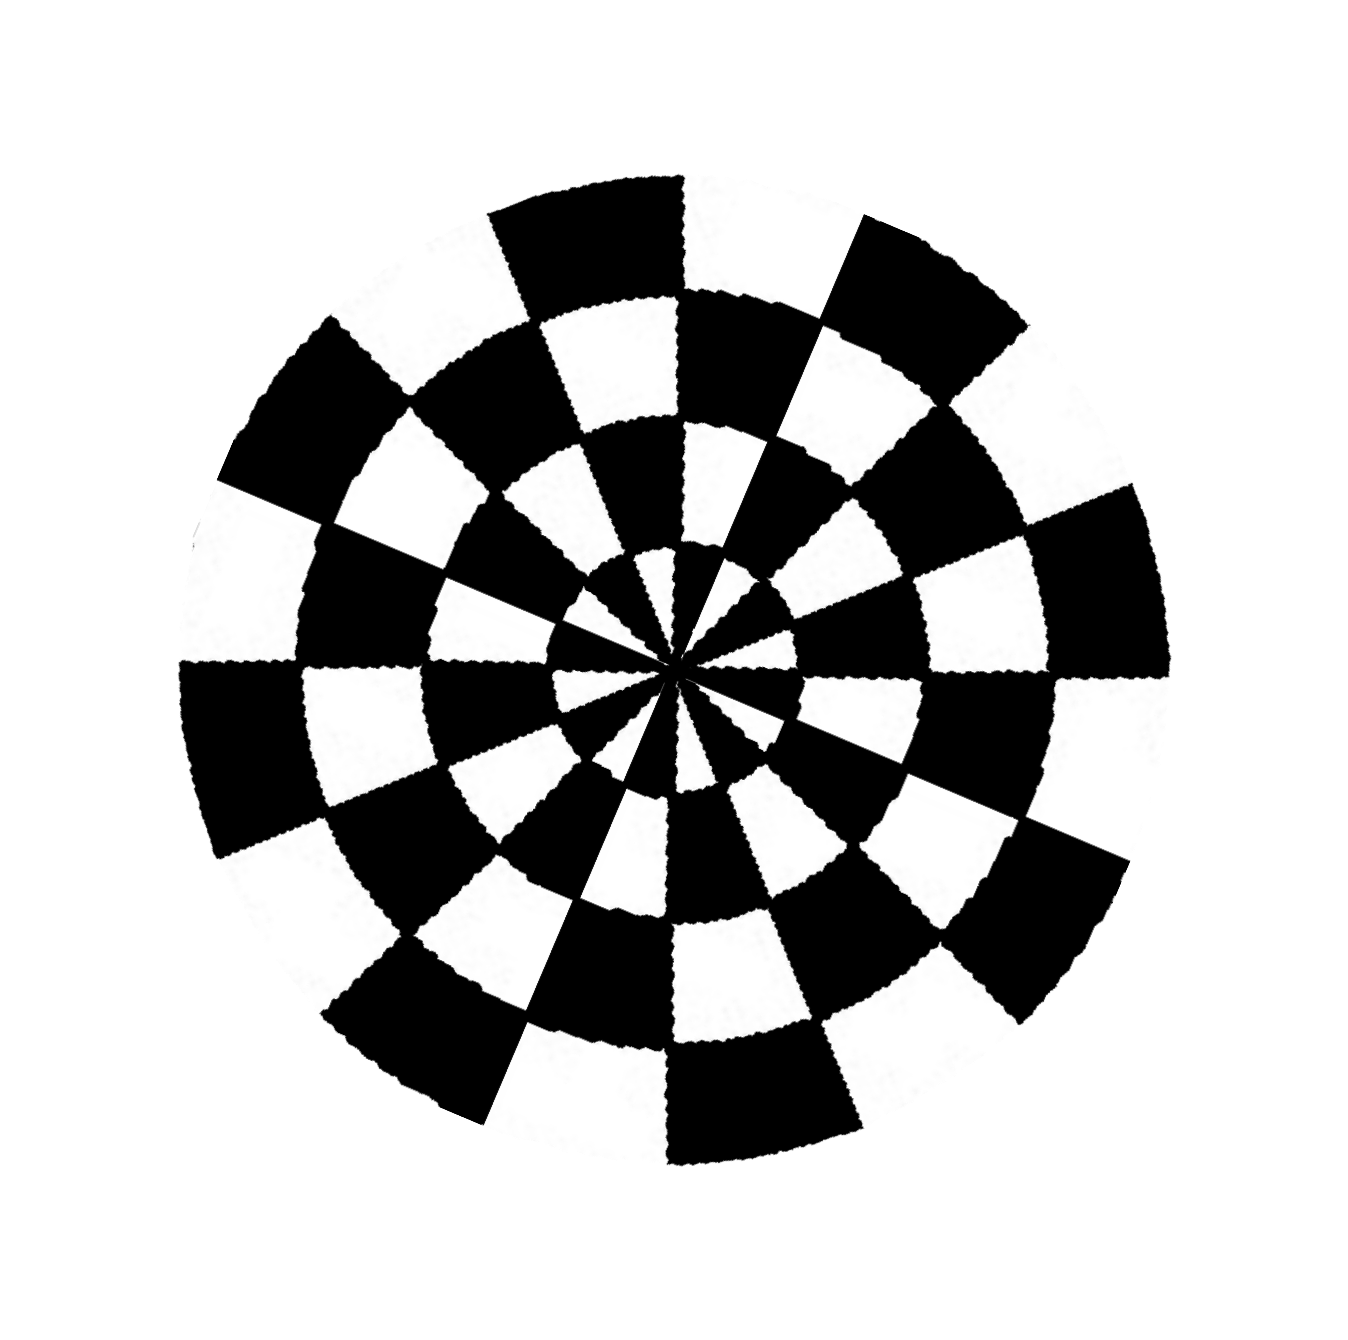
\includegraphics[width=2cm,height=2cm]{experiments/pattern.png}}
    
    ;
    
    \draw [color=white, ultra thick]
    (0,2) -- (3,2) node[above,midway] { 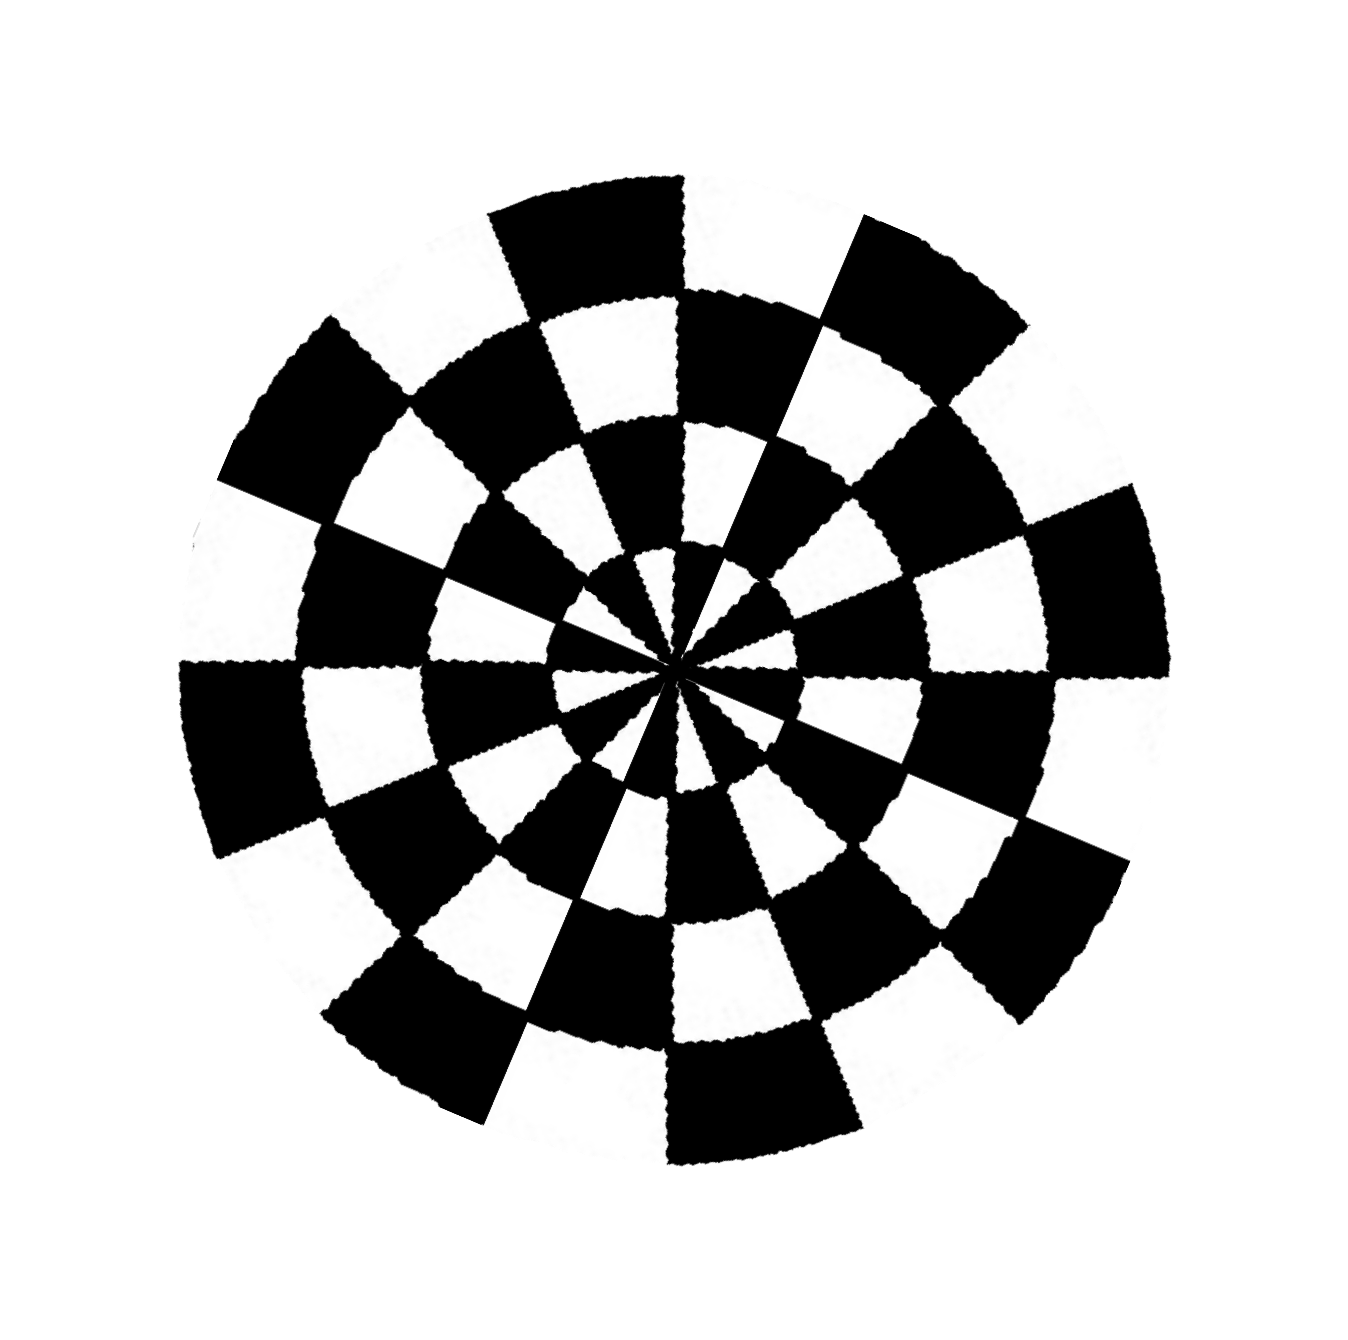
\includegraphics[width=2cm,height=2cm]{experiments/pattern.png}}
    (3,2) -- (6,2) node[above,midway] {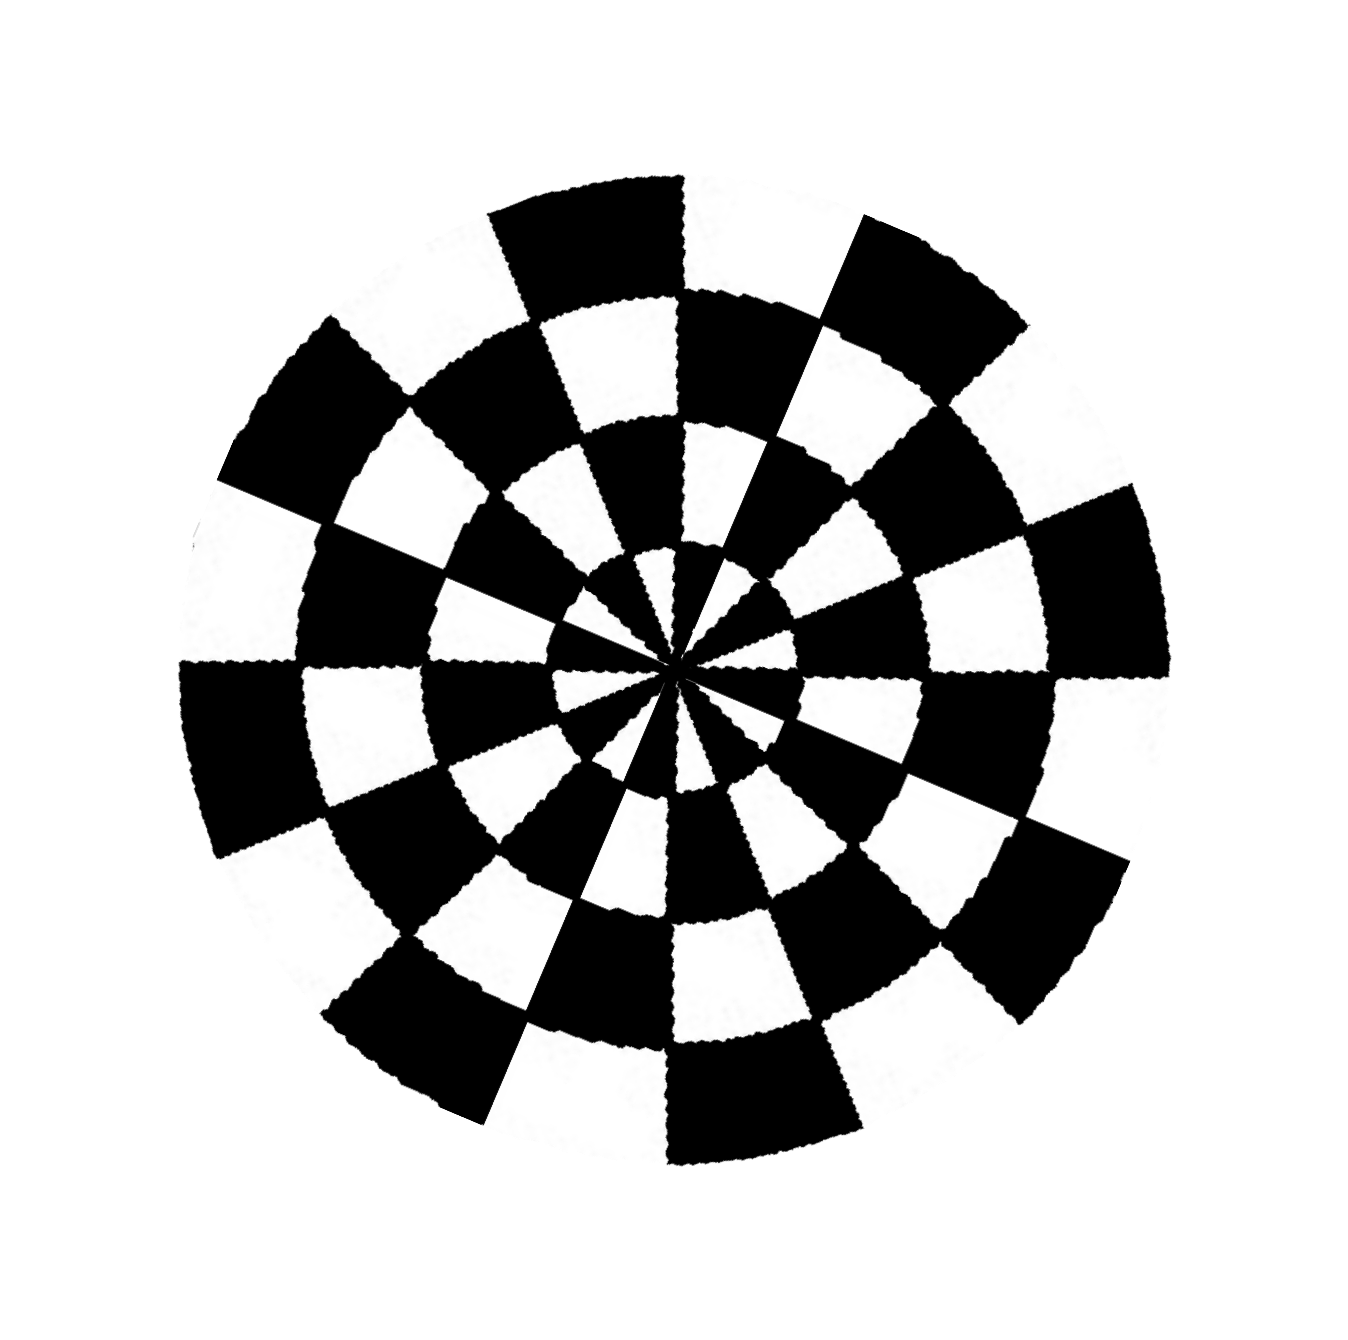
\includegraphics[width=2cm,height=2cm]{experiments/pattern.png}} 
    (6,2) -- (9,2) node[above, midway] {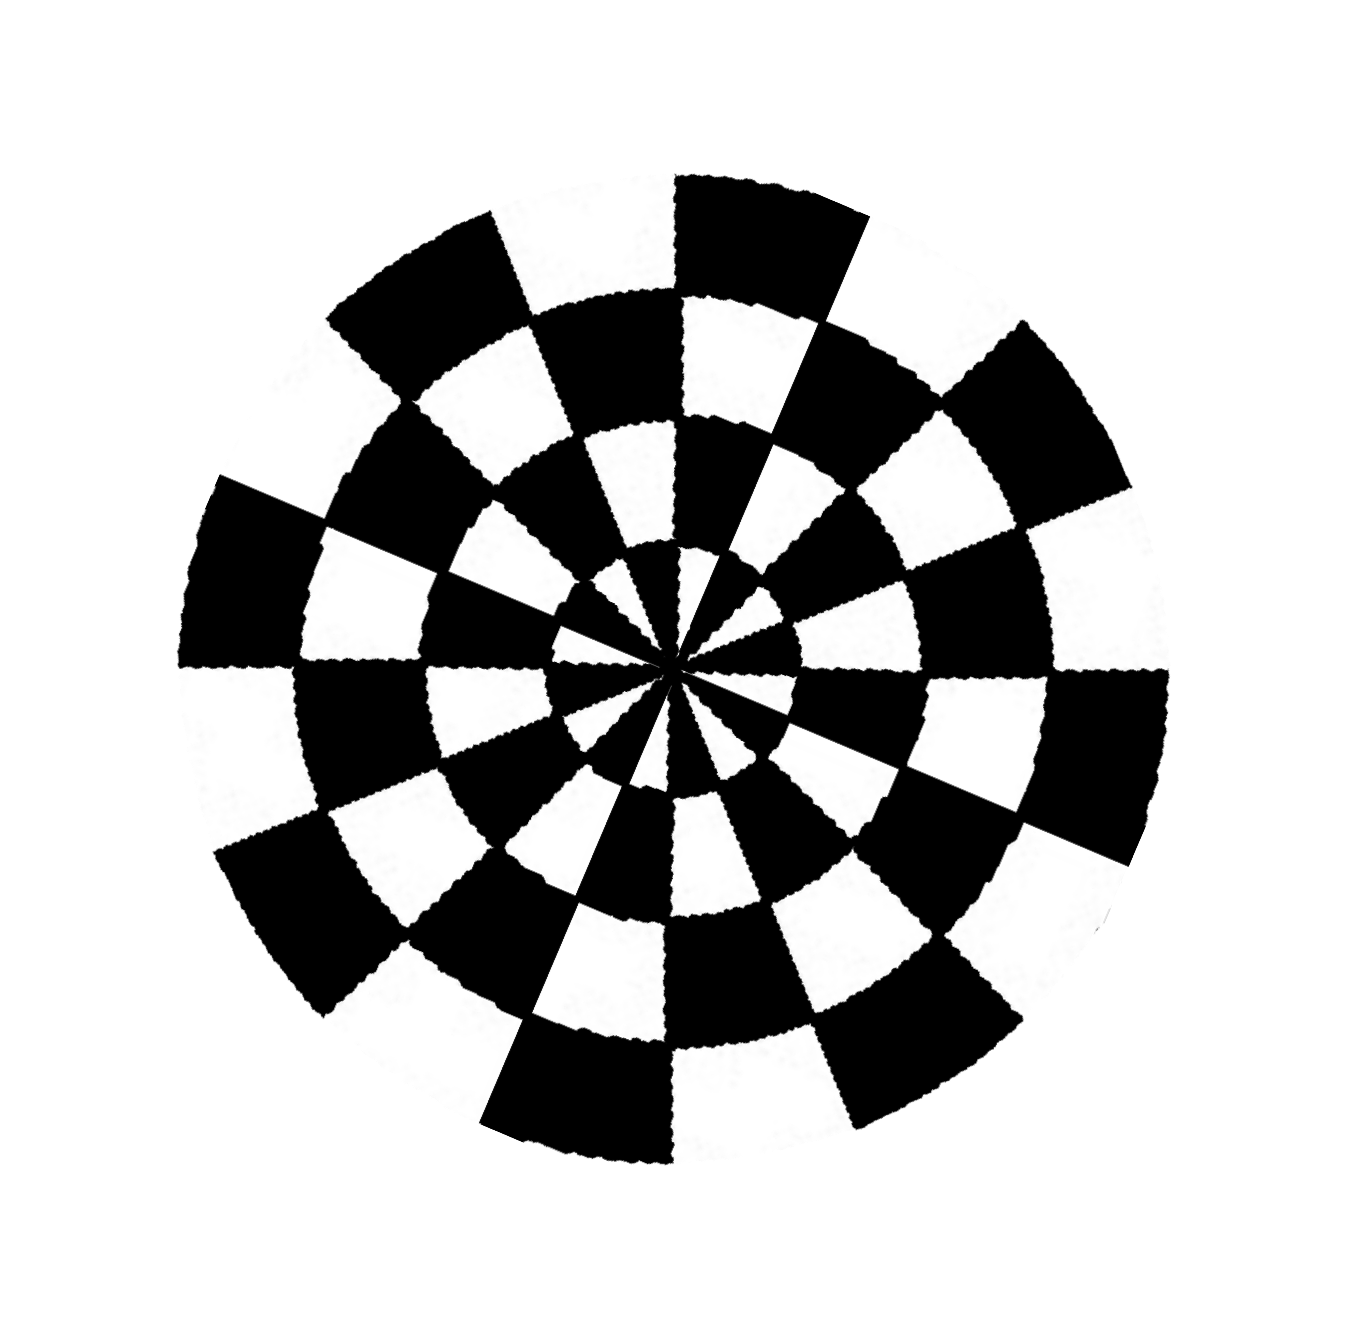
\includegraphics[width=2cm,height=2cm]{experiments/pattern_f.png}}
    (9,2) -- (12,2) node[above, midway] {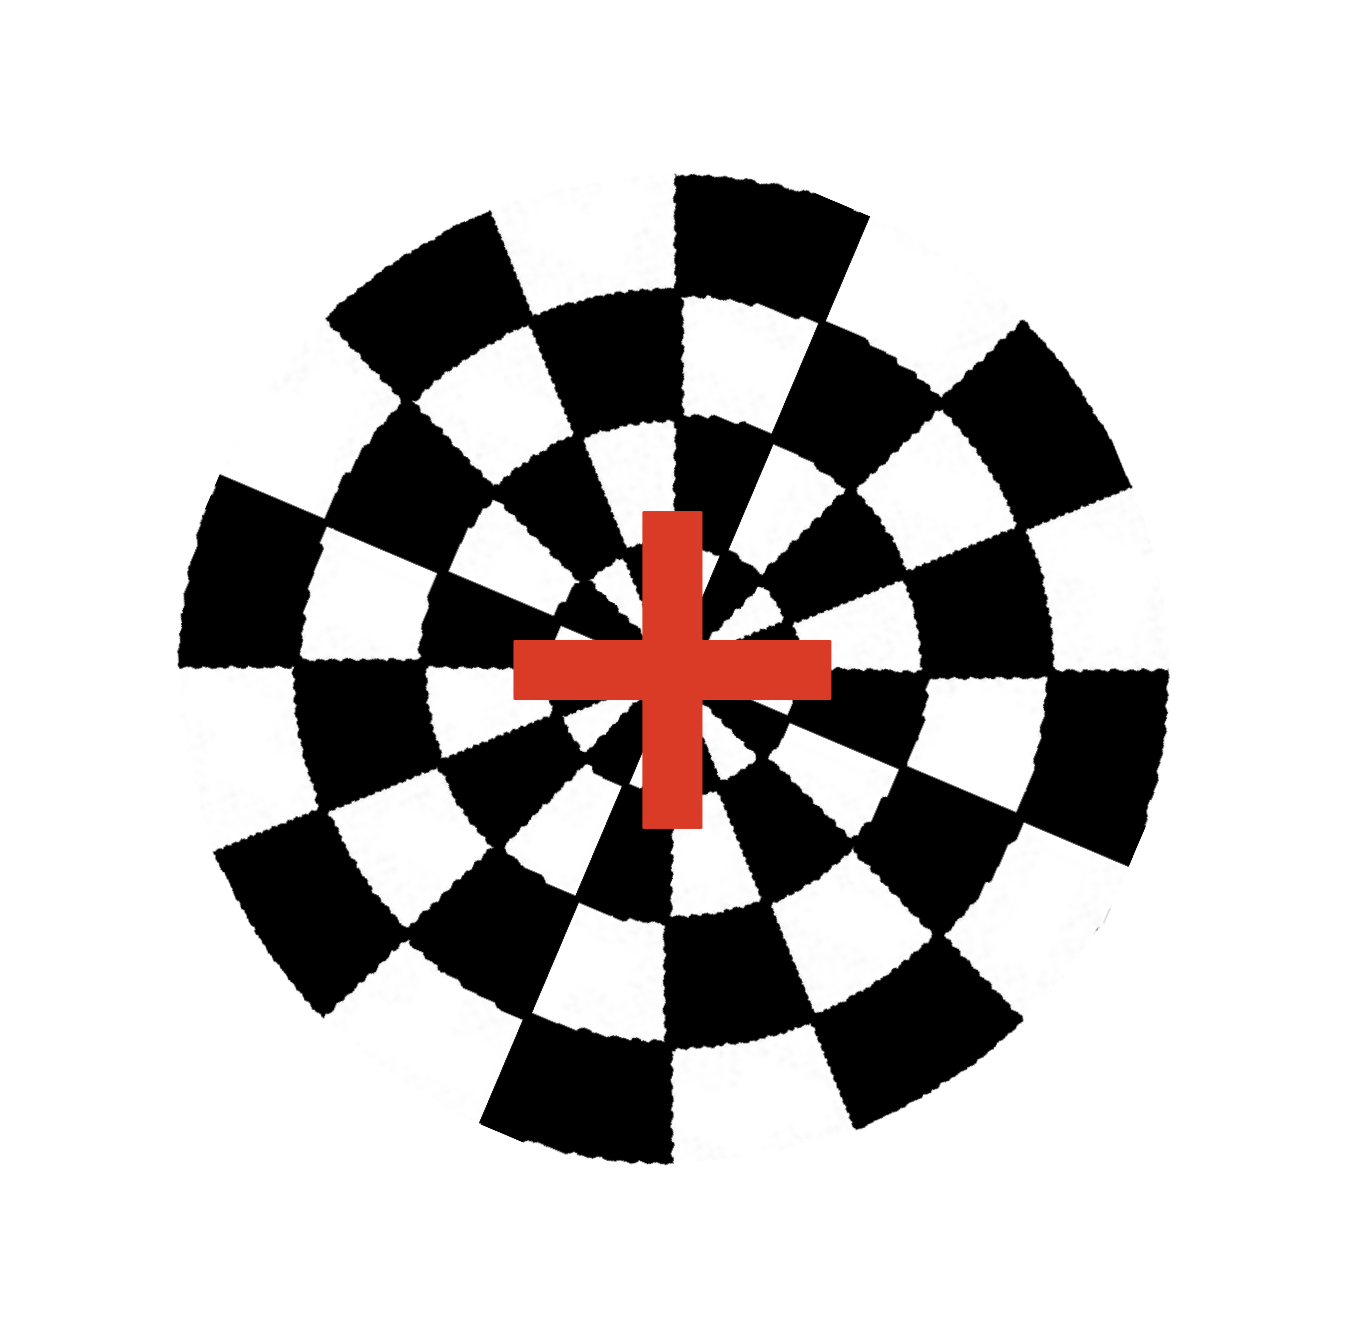
\includegraphics[width=2cm,height=2cm]{experiments/pattern_cross.png}}
    ;
    
    \draw[color=white, ultra thick]
    (0,4) -- (3,4) node[above,midway] { 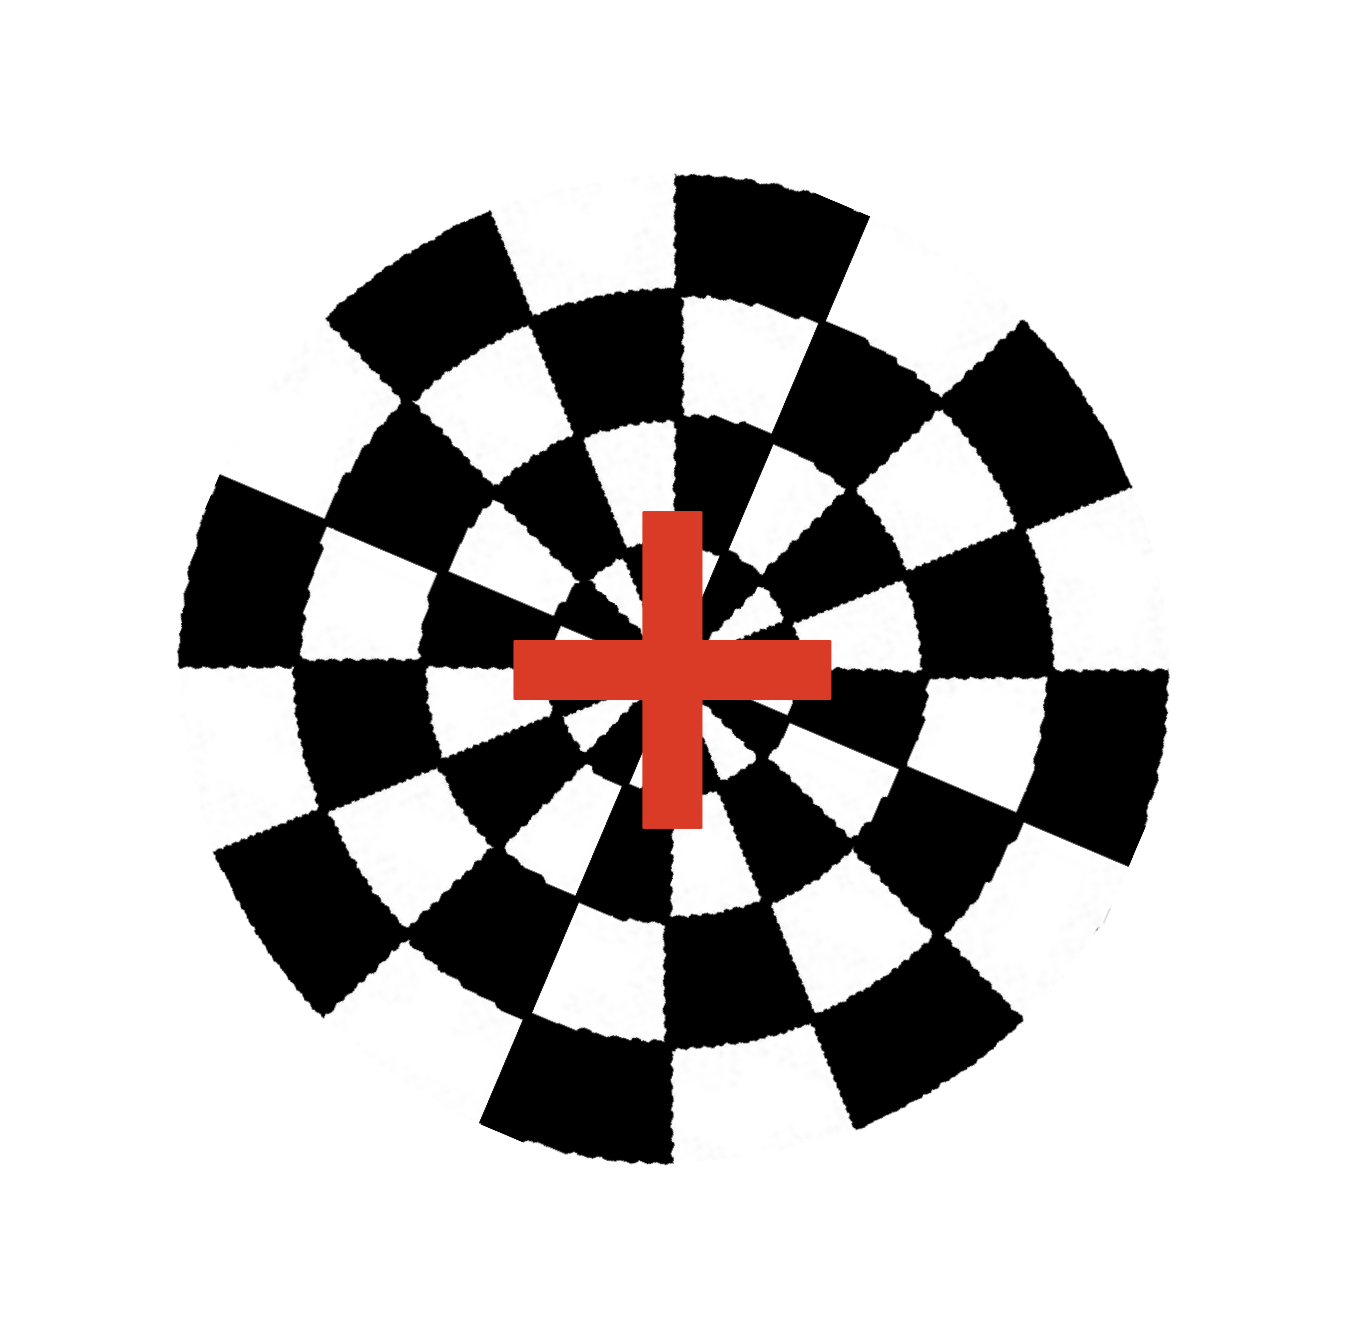
\includegraphics[width=2cm,height=2cm]{experiments/pattern_cross.png}}
    (3,4) -- (6,4) node[above,midway] {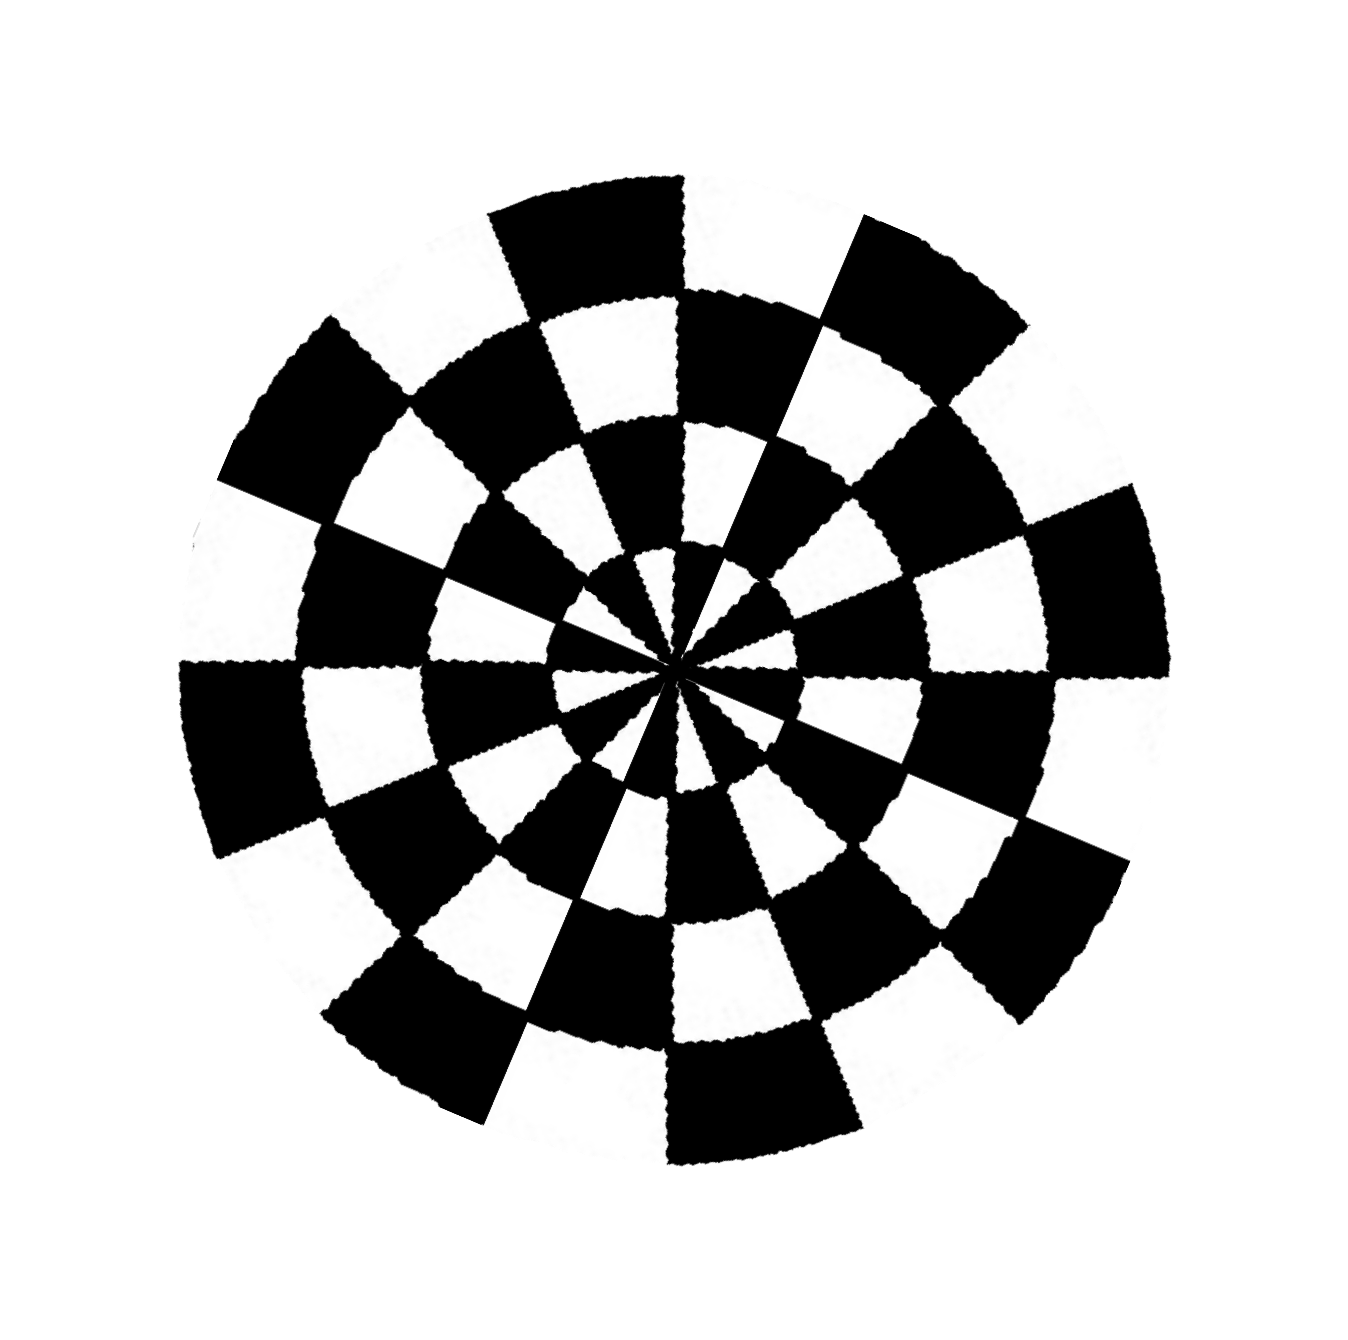
\includegraphics[width=2cm,height=2cm]{experiments/pattern.png}} 
    (6,4) -- (9,4) node[above, midway] {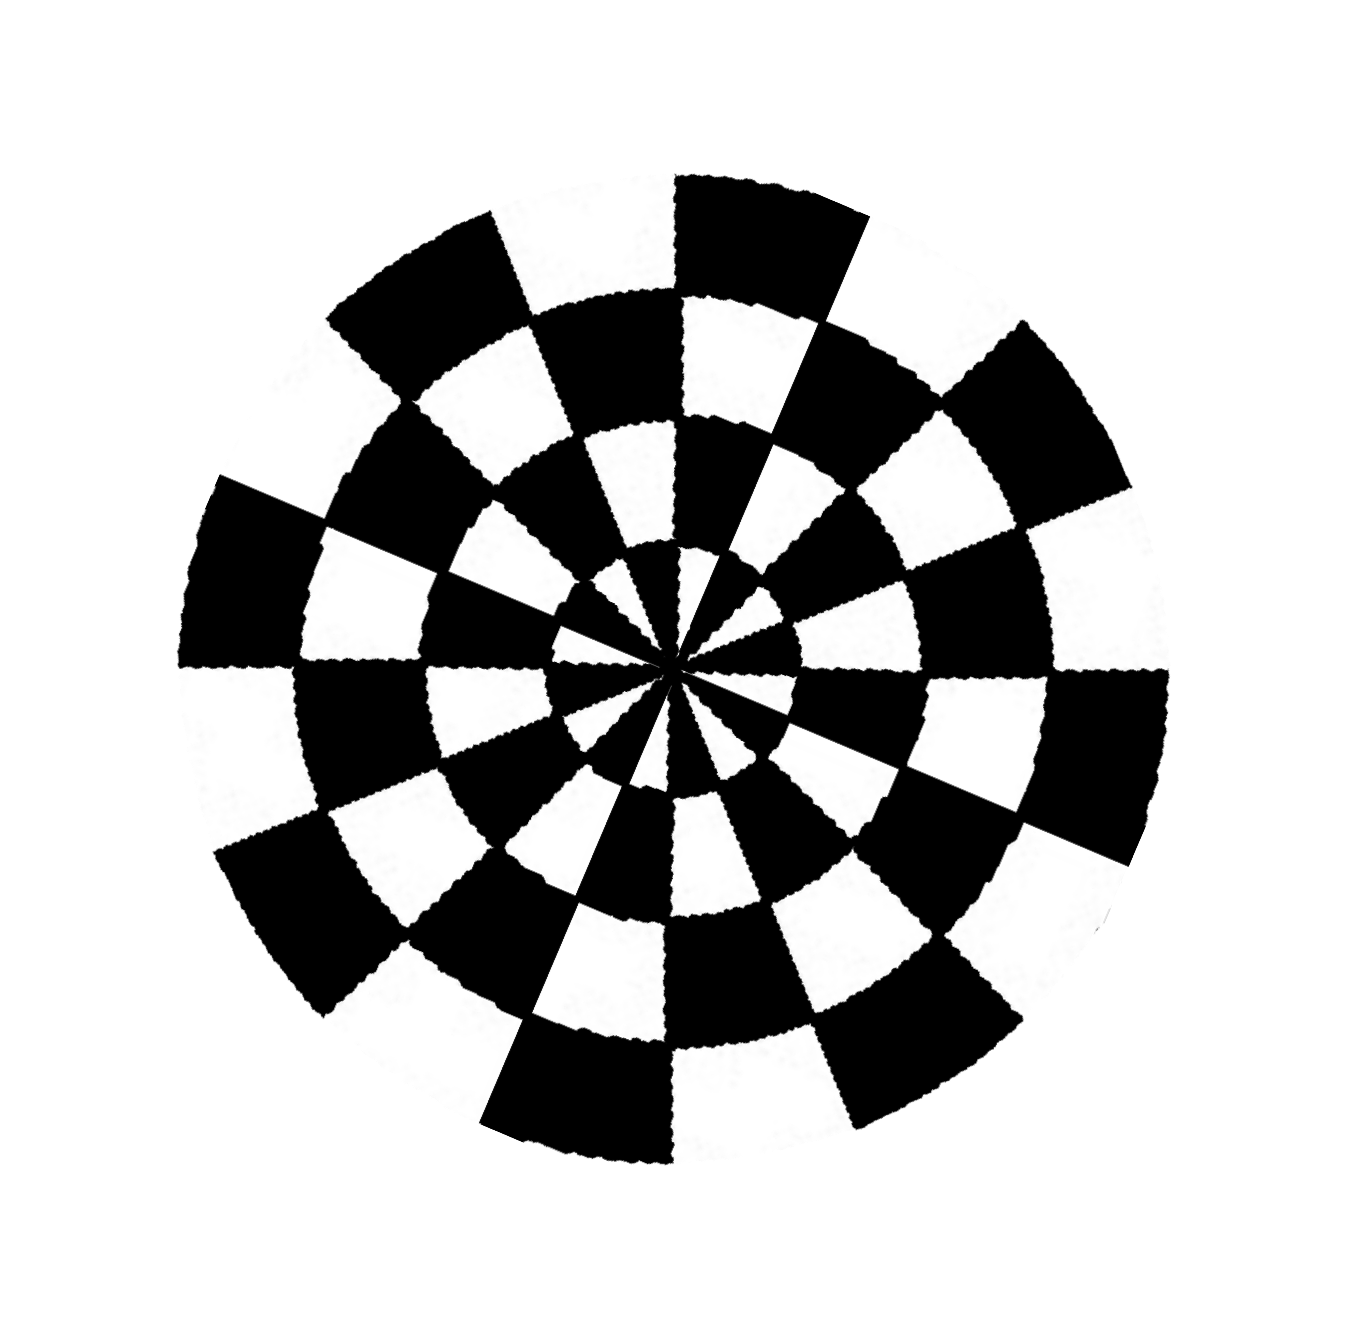
\includegraphics[width=2cm,height=2cm]{experiments/pattern_f.png}}
    (9,4) -- (12,4) node[above, midway] {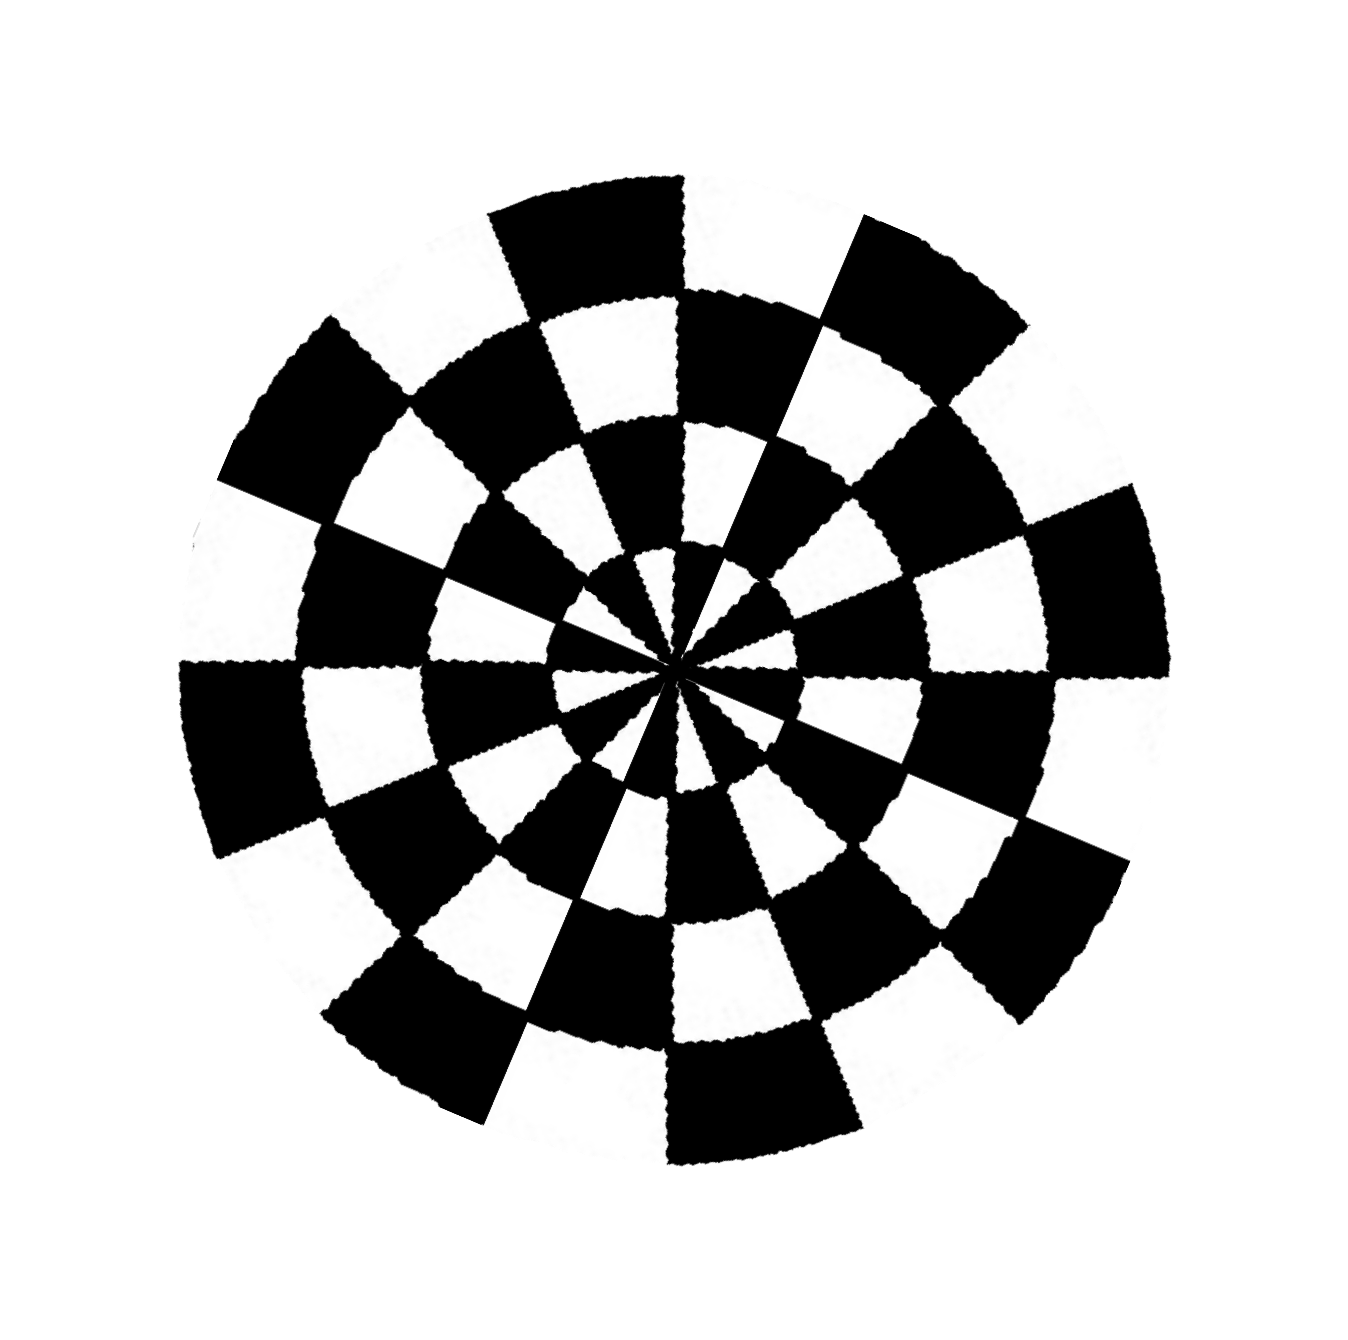
\includegraphics[width=2cm,height=2cm]{experiments/pattern.png}}
    ;

    \draw[color=white, ultra thick] (12,0) --(13,0);
    \draw[color=white, ultra thick] (12,2) --(13,2);
    \draw[color=white, ultra thick] (12,4) --(13,4);
    
    % add SSVEP label on top of arrow
    \node[above] at (6,2.8) {SSVEP};
    \draw[ultra thick, ->] (5.5,2.75) -- (6.5,2.75);
    
    \node[above] at (6,4.8) {SSVEP};
    \draw[ultra thick, ->] (5.5,4.75) -- (6.5,4.75);
    
    \node[above] at (6,0.8) {SSVEP};
    \draw[ultra thick, ->] (5.5,0.75) -- (6.5,0.75);
    \node[below] at (6,-0.5) {time (s)};
    
    \node[above] at (1.5,6.25) { \textbf{SSVEP Paused} };
    \node[above] at (10.5,6.25) { \textbf{SSVEP Paused} };
    \node[above] at (6,6.25) { \textbf{SSVEP On} };

    \node at (6,5.55) { Participant Fixated on Target 0};

    \node at (1.5,5.5) { Cross on Target 0};
    \node at (10.5,3.5) {Cross on Target 1};
    \draw[ultra thick, ->] (0,0) -- (13,0);

\end{tikzpicture}
\end{document}